%!TEX root = /Users/jakubkonka/Thesis/Thesis.tex
\chapter{Static Analysis of Network Selection Mechanism: Indirect Approach}
\label{cha:indirect}

\minitoc
\vspace{10mm}

In this chapter, the bidding problem described in Section~\ref{sec:problem_definition_and_assumptions_direct} will be transformed from a bidding problem with symmetric type (or cost) distributions into a bidding problem with asymmetric type distributions. This type of bidding problems has already been researched by the economic community, both in a very specific setting (two bidders, specific type distributions) \cite{KaplanZamir2007,MaskinRiley2000}, and in a very general setting ($n$ bidders, arbitrary type distributions) \cite{Lebrun1999,Lebrun2006}, and hence there exist results that are applicable to the problem at hand.

In order to transform the problem, recall the utility function for each network operator $i$
\begin{equation*}
  u_i(b,c,r) = \left\{
  \begin{array}{l l}
    b_i-c_i & \;\text{if } wb_i + (1-w)r_i < \displaystyle\min_{j\neq i}[wb_j + (1-w)r_j],\\
    0 & \;\text{if } wb_i + (1-w)r_i > \displaystyle\min_{j\neq i}[wb_j + (1-w)r_j],
  \end{array}\right.
\end{equation*}
and let
\begin{equation}
  \label{eq:b_hat_indirect}
  \hat{b}_i = wb_i + (1-w)r_i \quad\text{for all } i\in N.
\end{equation}
(Note that the new bid is just an alias for the compound bid, and in fact, they are equivalent; $\beta(b_i,r_i)\equiv\hat{b}_i$.) Solving Equation~\eqref{eq:b_hat_indirect} for $b_i$ yields
\begin{equation}
  \label{eq:b_from_b_hat_indirect}
  b_i = \frac{\hat{b}_i - (1-w)r_i}{w}, \quad w\neq 0.
\end{equation}
Substituting Equation~\eqref{eq:b_from_b_hat_indirect} back into the utility function yields
\begin{equation*}
  u_i(\hat{b},c,r) = \left\{
  \begin{array}{l l}
    \displaystyle\frac{1}{w}\left[\hat{b}_i-(wc_i + (1-w)r_i)\right] & \;\text{if } \hat{b}_i < \displaystyle\min_{j\neq i}\hat{b}_j,\\[2ex]
    0 & \;\text{if } \hat{b}_i > \displaystyle\min_{j\neq i}\hat{b}_j.
  \end{array}\right.
\end{equation*}
If we further let
\begin{equation}
  \label{eq:cost_hat_indirect}
  \hat{c}_i = wc_i + (1-w)r_i \quad\text{for all } i\in N,
\end{equation}
the utility function simplifies to
\begin{equation}
  \label{eq:sellers_utility_hat_indirect}
  u_i(\hat{b},\hat{c}) = \left\{
  \begin{array}{l l}
    \displaystyle\frac{1}{w}\left(\hat{b}_i-\hat{c}_i\right) & \;\text{if } \hat{b}_i < \displaystyle\min_{j\neq i}\hat{b}_j,\\[2ex]
    0 & \;\text{if } \hat{b}_i > \displaystyle\min_{j\neq i}\hat{b}_j.
  \end{array}\right.
\end{equation}
In order to avoid ambiguity, we shall refer to $\hat{c}_i$ as costs-hat and $\hat{b}_i$ as bids-hat, while still referring to $c_i$ as costs and $b_i$ as bids. Note, moreover, that since both $w$ and $r_i$ are assumed to be given to the network operators (i.e., they cannot directly modify their values), the costs-hat and bids-hat are simply convex (and hence, linear) combinations involving costs and bids respectively (Equations~\eqref{eq:b_hat_indirect}~and~\eqref{eq:cost_hat_indirect}). Therefore, a network operator bidding their cost-hat is equivalent to bidding their cost.

As a result of this transformation, the costs-hat, $\hat{c}_i$, for each network operator $i$ are distributed over the interval
\begin{equation*}
  \hat{c}_i\in [(1-w)r_i, (1-w)r_i + w]
\end{equation*}
since $c_i\in [0,1]$ for all $i\in N$. Note, moreover, that for all $i\in N$
\begin{equation*}
  [(1-w)r_i, (1-w)r_i + w] \subset [0,1]
\end{equation*}
since $w\in (0,1)$ and $r_i\in [0,1]$, and in particular, if $w=1$
\begin{equation*}
  [(1-w)r_i, (1-w)r_i + w] = [0,1].
\end{equation*}

With these results at hand, we can proceed with the analysis of the game.

\section{Generic Case} % (fold)
\label{sec:generic_case_indirect}
In the generic case, with arbitrary probability distributions of costs and $n\ge 2$ network operators, recall that: if $w=0$, then Proposition~\ref{prop:special_case_w_0_direct} holds; if $w=1$, then Proposition~\ref{prop:special_case_w_1_direct} holds; and if $r_i=r_j$ for all $i,j\in N$ such that $i\neq j$, then Corollary~\ref{cor:special_case_r_i_r_j_direct} holds. Therefore, it is sufficient to consider only the case when $w\in(0,1)$, and at least one network operator is characterized by a different reputation rating from the other network operators; that is, there exists $i\in N$ such that $r_i\neq r_j$ for all $i\neq j$ and $j\in N$.

Firstly, note that under the generic assumptions specified in Section~\ref{sec:problem_definition_and_assumptions_direct}, the problem satisfies the following regularity conditions.
\begin{proposition}[Regularity Conditions]
\label{prop:regularity_conditions_indirect}
Let $F_i$ be the distribution function of $\hat{c}_i$ for all $i\in N$. Then,
\begin{enumerate}
  \item the support of $F_i$ is an interval ${[(1-w)r_i, (1-w)r_i + w]}$;
  \item $F_i$ is differentiable over ${((1-w)r_i, (1-w)r_i + w]}$ with a derivative $f_i$ locally bounded away from zero over this interval; and
  \item $F_i$ is atomless.
\end{enumerate}
\end{proposition}

The regularity conditions in Proposition~\ref{prop:regularity_conditions_indirect} correspond to the regularity assumptions on type distributions put forward by Lebrun~\cite{Lebrun2006} (cf. Assumptions~A.1 in~\cite{Lebrun2006}). Therefore, since our problem satisfies Lebrun's assumptions, his results are applicable to our problem, and we conclude that:
\begin{proposition}[Characterization of the Equilibrium]
\label{prop:characterisation_of_the_equilibrium_indirect}
$\quad$\\
\begin{enumerate}
  \item There exists a pure-strategy Bayesian Nash equilibrium where network operators submit at least their costs, and
  \item the pure-strategy Bayesian Nash equilibrium where network operators submit at least their costs is unique.
\end{enumerate}
\end{proposition}

However, even though the equilibrium exists and is unique, the establishment of a closed-form solution in a generic setting ($n\ge 2$ network operators and arbitrary cost distribution) is very difficult (if even possible) \cite{Lebrun2006, Krishna10}.
% section indirect_generic_case (end)

\section{Restricted Case $n=2$} % (fold)
\label{sec:restricted_case_n_2_indirect}
It is possible to explicitly derive the equilibrium bidding strategy functions in a much restricted setting. Let $n=2$ network operators, and assume costs, $c_i$, for both network operators are drawn from the uniform distribution. The utility function becomes
\begin{equation*}
  u_i(\hat{b},\hat{c}) = \left\{
  \begin{array}{l l}
    \displaystyle\frac{1}{w}\left(\hat{b}_i-\hat{c}_i\right) & \;\text{if } \hat{b}_i < \hat{b}_j,\\[2ex]
    \displaystyle\frac{1}{2w}\left(\hat{b}_i-\hat{c}_i\right) & \;\text{if } \hat{b}_i = \hat{b}_j,\\[2ex]
    0 & \;\text{if } \hat{b}_i > \hat{b}_j.
  \end{array}\right.
\end{equation*}
Without loss of generality, suppose $r_i < r_j$. Since the distribution of costs, $c_i$, for each network operator $i$ is uniform with the support $[0,1]$, Equation~\eqref{eq:cost_hat_indirect} implies that the distribution of costs-hat, $\hat{c}_i$, for each network operator $i$ is uniform with the support~${[\underline{\hat{c}}_i, \bar{\hat{c}}_i]} = {[(1-w)r_i, (1-w)r_i + w]}$. Therefore, the distribution function of costs-hat satisfies the regularity conditions specified in Proposition~\ref{prop:regularity_conditions_indirect}, and by Proposition~\ref{prop:characterisation_of_the_equilibrium_indirect}, we conclude that the pure-strategy Bayesian Nash equilibrium where network operators submit at least their costs exists and is unique.

The derivation of the equilibrium involves three stages: 1) deriving equilibrium inverse bidding strategy functions using the procedure described by Kaplan and Zamir~\cite{KaplanZamir2007}; 2) numerically estimating the equilibrium bidding strategy functions by inverting the inverses; and 3) transforming the problem back to the original domain (from costs-hat and bids-hat back to costs and bids). Since $r_i < r_j$, this implies that $\bar{\hat{c}}_i < \bar{\hat{c}}_j$. It is, moreover, assumed that bids are bounded from above which implies that no network operator wins by bidding more than $\bar{\hat{c}}_j$ (since $\bar{\hat{c}}_i < \bar{\hat{c}}_j$). In particular, in equilibrium, there is no bid higher than $\bar{\hat{c}}_j$. Furthermore, it is assumed that, in equilibrium, a network operator with zero probability of winning bids their cost-hat. (This assumption guarantees both the existence and uniqueness of the equilibrium by Proposition~\ref{prop:characterisation_of_the_equilibrium_indirect}.)

If $\bar{\hat{c}}_i \le 2\underline{\hat{c}}_j - \bar{\hat{c}}_j$, then any pure-strategy Bayesian Nash equilibrium must have network operator $i$ always bidding $\underline{\hat{c}}_j$, and hence, always winning the auction at price $\underline{\hat{c}}_j$. This case shall be referred to as trivial. Therefore, in the non-trivial case, we must have $\bar{\hat{c}}_i > 2\underline{\hat{c}}_j - \bar{\hat{c}}_j$ (cf. Lemma~1 in Kaplan and Zamir~\cite{KaplanZamir2007}). In this range, an equilibrium consists of strictly increasing, differentiable bidding strategy functions $\hat{b}_i(\hat{c})$ and $\hat{b}_j(\hat{c})$. Let the inverses of these bidding strategy functions be denoted as $\hat{c}_i(\hat{b})$ with support $[\underline{\hat{b}}_i, \bar{\hat{b}}_i]$, and $\hat{c}_j(\hat{b})$ with support $[\underline{\hat{b}}_j, \bar{\hat{b}}_j]$. As Kaplan and Zamir~\cite{KaplanZamir2007} establish, these supports are identical, and equal to the common support $[\underline{\hat{b}}, \bar{\hat{b}}]$.

Suppose, therefore, that $\bar{\hat{c}}_i > 2\underline{\hat{c}}_j - \bar{\hat{c}}_j$ holds, and consider the optimization problem for network operator $i$
\begin{align*}
  &\max_{b} E \left[ b - \hat{c}_i \:\middle\vert\: b < \hat{b}_j \right]\\
  = &\max_{b} (b - \hat{c}_i)\cdot P\{b < \hat{b}_j\}\\
  = &\max_{b} (b - \hat{c}_i)\cdot P\{\hat{c}_j(b) < \hat{C}_j\}\\
  = &\max_{b} (b - \hat{c}_i)(1 - F_j(\hat{c}_j(b)),
\end{align*}
where $F_j$ is the distribution function of costs-hat for network operator $j$. The first-order condition yields
\begin{align}
  &1 - F_j(\hat{c}_j(b)) - (b - \hat{c}_i)f_j(\hat{c}_j(b))\cdot\frac{d}{db}\hat{c}_j(b) = 0 \nonumber \\
  \iff &1 - \frac{\hat{c}_j(b) - \underline{\hat{c}}_j}{\bar{\hat{c}}_j - \underline{\hat{c}}_j} = \frac{1}{\bar{\hat{c}}_j - \underline{\hat{c}}_j}(b - \hat{c}_i)\cdot\frac{d}{db}\hat{c}_j(b) \nonumber \\
  \iff &(\hat{c}_i(b) - b)\cdot\frac{d}{db}\hat{c}_j(b) = \hat{c}_j(b) - \bar{\hat{c}}_j,
  \label{eq:first_order_bidder_i_indirect}
\end{align}
where we have used the facts that $F_j$ is the distribution function of the uniform distribution with the support $[\underline{\hat{c}}_j, \bar{\hat{c}}_j]$, and at an equilibrium $\hat{c}_i = \hat{c}_i(b)$. Similarly, for network operator $j$ we have
\begin{equation}
  \label{eq:first_order_bidder_j_indirect}
  (\hat{c}_j(b) - b)\cdot\frac{d}{db}\hat{c}_i(b) = \hat{c}_i(b) - \bar{\hat{c}}_i.
\end{equation}

The following boundary conditions must hold in equilibrium (cf. boundary conditions in Kaplan and Zamir~\cite{KaplanZamir2007}):
\begin{enumerate}
  \item $\hat{c}_j(\bar{\hat{b}}) = \bar{\hat{b}}$, (the network operator bids their cost-hat when their probability of winning is zero),
  \item $\hat{c}_i(\bar{\hat{b}}) = \bar{\hat{c}}_i$, (the maximum cost-hat that gives network operator $i$ a positive probability of winning), and
  \item $\hat{c}_i(\underline{\hat{b}}) = \underline{\hat{c}}_i$ and $\hat{c}_j(\underline{\hat{b}}) = \underline{\hat{c}}_j$ (the lowest bid-hat of each network operator is reached for their lowest cost-hat).
\end{enumerate}
Integrating Equations~\eqref{eq:first_order_bidder_i_indirect}~and~\eqref{eq:first_order_bidder_j_indirect} bounded by the aforementioned boundary conditions results in the derivation of the equilibrium inverse bidding strategy functions. The derivation procedure is fully described in Kaplan and Zamir~\cite{KaplanZamir2007}; hence, we only provide the final result.
\begin{proposition}
\label{prop:inverse_equi_bidding_str_indirect}
Let there be $n=2$ network operators, and suppose $c_i$ is independently drawn from uniform distribution over the interval $[0,1]$ for all $i\in N$. Let for all $i\in N$
\begin{equation*}
  \hat{b}_i = wb_i + (1-w)r_i,\quad\text{and}\quad \hat{c}_i = wc_i + (1-w)r_i,
\end{equation*}
with
\begin{equation}
  \label{eq:cost_hat_bounds_indirect}
  \underline{\hat{c}}_i = (1-w)r_i,\quad \bar{\hat{c}}_i = (1-w)r_i + w.
\end{equation}
Then the equilibrium inverse bidding strategy functions for all $i\in N$ and $w\in (0,1)$ are given by
\begin{align}
  \label{eq:inverse_equi_bidding_str_i_indirect}
  \hat{c}_i(b) &= \bar{\hat{c}}_i + \frac{(\bar{\hat{c}}_j - \bar{\hat{c}}_i)^2}{(\bar{\hat{c}}_j + \bar{\hat{c}}_i - 2b)d_i \exp{\left(\displaystyle\frac{\bar{\hat{c}}_j - \bar{\hat{c}}_i}{\bar{\hat{c}}_j + \bar{\hat{c}}_i - 2b}\right)} + 4(\bar{\hat{c}}_j - b)},\\[2ex]
  \label{eq:inverse_equi_bidding_str_j_indirect}
  \hat{c}_j(b) &= \bar{\hat{c}}_j + \frac{(\bar{\hat{c}}_i - \bar{\hat{c}}_j)^2}{(\bar{\hat{c}}_i + \bar{\hat{c}}_j - 2b)d_j \exp{\left(\displaystyle\frac{\bar{\hat{c}}_i - \bar{\hat{c}}_j}{\bar{\hat{c}}_i + \bar{\hat{c}}_j - 2b}\right)} + 4(\bar{\hat{c}}_i - b)},
\end{align}
where
\begin{align}
  \label{eq:constant_d_i_indirect}
  d_i = \frac{\displaystyle\frac{(\bar{\hat{c}}_j - \bar{\hat{c}}_i)^2}{\underline{\hat{c}}_i - \bar{\hat{c}}_i} + 4(\underline{\hat{b}} - \bar{\hat{c}}_j)}{-2(\underline{\hat{b}} - \bar{\hat{b}})} \exp{\left(\displaystyle\frac{\bar{\hat{c}}_j - \bar{\hat{c}}_i}{2(\underline{\hat{b}} - \bar{\hat{b}})}\right)}, \\[2ex]
  \label{eq:constant_d_j_indirect}
  d_j = \frac{\displaystyle\frac{(\bar{\hat{c}}_i - \bar{\hat{c}}_j)^2}{\underline{\hat{c}}_j - \bar{\hat{c}}_j} + 4(\underline{\hat{b}} - \bar{\hat{c}}_i)}{-2(\underline{\hat{b}} - \bar{\hat{b}})} \exp{\left(\frac{\bar{\hat{c}}_i - \bar{\hat{c}}_j}{2(\underline{\hat{b}} - \bar{\hat{b}})}\right)},
\end{align}
and
\begin{equation}
  \label{eq:bid_bounds_indirect}
  \underline{\hat{b}} = \frac{\underline{\hat{c}}_i\underline{\hat{c}}_j - \displaystyle\frac{(\bar{\hat{c}}_i + \bar{\hat{c}}_j)^2}{4}}{\underline{\hat{c}}_i - \bar{\hat{c}}_i + \underline{\hat{c}}_j - \bar{\hat{c}}_j},\quad
  \bar{\hat{b}} = \frac{\bar{\hat{c}}_i + \bar{\hat{c}}_j}{2}.
\end{equation}
\end{proposition}
Note that the equilibrium inverse bidding strategy functions are inconvenient to work with: for a particular bid-hat value, they map into a particular cost-hat for either network operator. It would be more intuitive to work with their inverses, where for a particular cost-hat, we would get a particular bid-hat. Since it is difficult (if even possible) to analytically invert the equilibrium inverse bidding strategy functions in Equations~\eqref{eq:inverse_equi_bidding_str_i_indirect}~and~\eqref{eq:inverse_equi_bidding_str_j_indirect}, we resort to numerical methods for estimating the inverses for a particular set of cost-reputation pairs with respect to the price weights for both network operators. Without loss of generality, assume that $r_i < r_j$. The numerical procedure is then as follows.
\begin{enumerate}
  \item For a particular price weight $w$ and reputation ratings $r_i$ and $r_j$, calculate the costs-hat supports for both network operators; that is, the endpoints of the interval $[\underline{\hat{c}}_i, \bar{\hat{c}}_i]$ for network operator $i$, and $[\underline{\hat{c}}_j, \bar{\hat{c}}_j]$ for network operator $j$ (Equation~\eqref{eq:cost_hat_bounds_indirect}).
  \item If $\bar{\hat{c}}_i \le 2\underline{\hat{c}}_j - \bar{\hat{c}}_j$, then the equilibrium is trivial. Network operator $i$ bids the lower endpoint of the cost-hat support of network operator $j$; that is, network operator $i$ bids $\underline{\hat{c}}_j$ for all $\hat{c}\in [\underline{\hat{c}}_i, \bar{\hat{c}}_i]$. Network operator $j$, on the other hand, bids their cost-hat; that is, network operator $j$ bids $\hat{c}$ for all $\hat{c}\in [\underline{\hat{c}}_j, \bar{\hat{c}}_j]$.
  \item If $\bar{\hat{c}}_i > 2\underline{\hat{c}}_j - \bar{\hat{c}}_j$, then the equilibrium is nontrivial. Hence,
  \begin{enumerate}
    \item Calculate the common bids-hat support $[\underline{\hat{b}}, \bar{\hat{b}}]$ (Equation~\eqref{eq:bid_bounds_indirect}).
    \item For all $\hat{b}\in [\underline{\hat{b}}, \bar{\hat{b}}]$, calculate the corresponding costs-hat for both network operators using Equations~\eqref{eq:inverse_equi_bidding_str_i_indirect}~and~\eqref{eq:inverse_equi_bidding_str_j_indirect}.
    \item Since by assumption $r_i < r_j$, it follows that $\bar{\hat{c}}_i \le \bar{\hat{c}}_j$, and hence, $\bar{\hat{b}}\le \bar{\hat{c}}_j$. Thus, network operator $j$ bids their cost-hat, $\hat{c}_j(\hat{b}) = \hat{c}_j$  for all $\hat{b}\in [\bar{\hat{b}}, \bar{\hat{c}}_j]$.
  \end{enumerate}
\end{enumerate}

\begin{figure}[p!]
  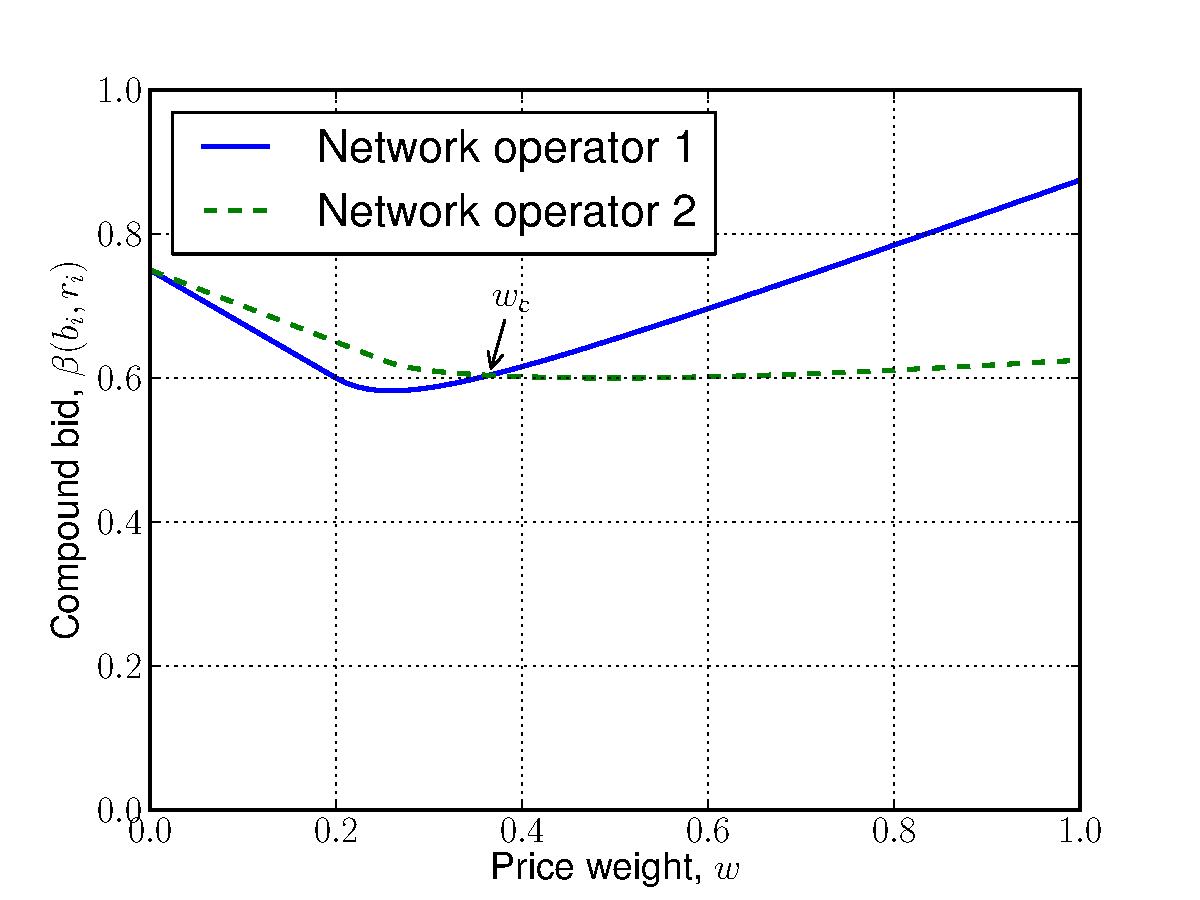
\includegraphics[width=\figsize]{Indirect/Figures/indirect_bids}
  \caption{Compound bid plotted against the price weight}
  \label{fig:indirect_bids_indirect}
  \vspace{10mm}
  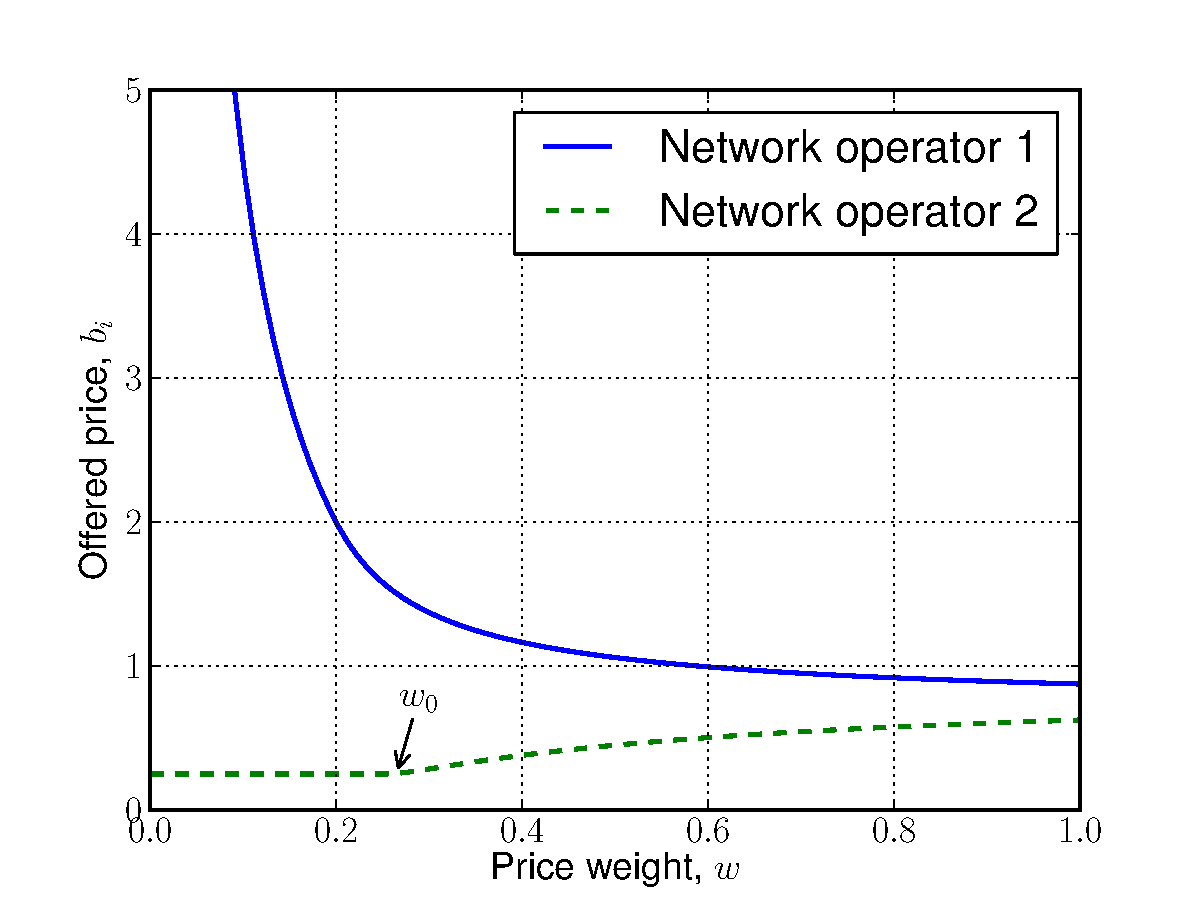
\includegraphics[width=\figsize]{Indirect/Figures/indirect_prices}
  \caption{Offered prices (bids) plotted against the price weight}
  \label{fig:indirect_prices_indirect}
\end{figure}

The result of the steps described above is the tabulation of the costs-hat and their corresponding equilibrium bids-hat for a particular price weight $w$, and reputation ratings $r_i$ and $r_j$ for both network operators, in the ranges $[\underline{\hat{c}}_i, \bar{\hat{c}}_i]$ for network operator $i$ and $[\underline{\hat{c}}_j, \bar{\hat{c}}_j]$ for network operator $j$. Denote by
\begin{equation}
  \label{eq:equi_bidding_str_i_indirect}
  \hat{b}_i(\hat{c}_i) = \hat{b}_i \quad\text{for all } \hat{c}_i\in[\underline{\hat{c}}_i, \bar{\hat{c}}_i],
\end{equation}
and
\begin{equation}
  \label{eq:equi_bidding_str_j_indirect}
  \hat{b}_j(\hat{c}_j) = \hat{b}_j \quad\text{for all } \hat{c}_j\in[\underline{\hat{c}}_j, \bar{\hat{c}}_j]
\end{equation}
the resultant equilibrium bidding strategy functions.

The problem can be transformed back into the original domain by substituting Equations~\eqref{eq:b_hat_indirect}~and~\eqref{eq:cost_hat_indirect} into Equations~\eqref{eq:equi_bidding_str_i_indirect}~and~\eqref{eq:equi_bidding_str_j_indirect}; that is,
\begin{equation*}
  \hat{b}_i(\hat{c}_i) = \hat{b}_i \iff b_i = \displaystyle\frac{\hat{b}_i(wc_i + (1-w)r_i) - (1-w)r_i}{w}
\end{equation*}
for all $c_i\in[0,1]$, and
\begin{equation*}
  \hat{b}_j(\hat{c}_j) = \hat{b}_j \iff b_j = \displaystyle\frac{\hat{b}_j(wc_j + (1-w)r_j) - (1-w)r_j}{w}
\end{equation*}
for all $c_j\in[0,1]$.
Keeping costs and reputation ratings fixed, one can then estimate the equilibrium bidding strategy functions with respect to the price weights by sliding the value of $w\in(0,1)$.

By way of example, the equilibrium bidding strategy functions were estimated for the set of cost-reputation pairs depicted in Table~\ref{tab:pcomp_direct}. Figure~\ref{fig:indirect_bids_indirect} shows the value of the compound bid, $\beta(b_i,r_i)$, for different values of $w$ for both network operators, while Figure~\ref{fig:indirect_prices_indirect} depicts the value of the monetary bid (or offered price), $b_i$, for different values of $w$ for both network operators. The numerical data in Table~\ref{tab:pcomp_direct} suggests that network operator 2 should be the winner for the values of $w\rightarrow 1$ since network operator 2's cost is strictly lower than that of their opponent's. On the other hand, network operator 1 should be winner for the values of $w\rightarrow 0$ since network operator 1's reputation rating is strictly lower than that of their opponent's (which implies that network operator 1's reputation is in fact strictly higher than that of their opponent's). This prediction agrees with the numerical output shown in Figure~\ref{fig:indirect_bids_indirect}. Let $w_c$ denote the value of $w$ for which an intersection between the compound bids of both network operators occurs (if it exists). In Figure~\ref{fig:indirect_bids_indirect}, $w_c\approx 0.365$. Hence, network operator 2 wins the auction for the values of $w_c < w < 1$, while network operator 1 for the values of $0 < w < w_c$.

Note, furthermore, that since we have explicitly required the network operators to bid their own costs when their probability of winning is zero, the monetary bid of network operator 2 is capped at their cost, $b_2 = 0.25$, for the values of $0 < w \le w_0$ where $w_0\approx 0.265$ (Figure~\ref{fig:indirect_prices_indirect}). In the same range of $w$, as $w$ decreases, network operator 1's bid increases in an exponential-like fashion, to finally culminate in $b_1\to\infty$ at $w=0$ in accordance with Proposition~\ref{prop:special_case_w_0_direct}. As $w\to 1$, on the other hand, the monetary bids of both network operators tend to the values specified in Proposition~\ref{prop:special_case_w_1_direct}, that is, $b_1=0.875$ and $b_2=0.625$, to finally attain those values at $w=1$.
% section indirect_restricted_case_n_2_ (end)

\section{Discussion} % (fold)
\label{sec:discussion_indirect}
The aim of this section is twofold. First, the results from direct and indirect approaches are compared. Second, the prices the subscriber has to pay for each value of the price weight given a tuple of network operators' reputation ratings (in the restricted case) are examined.

\subsection{Comparison of Results from Direct and Indirect Approaches} % (fold)
\label{sub:comparison_of_results_from_direct_and_indirect_approaches_indirect}
If the network operators are assumed to submit at least their costs, then, in the restricted case, Proposition~\ref{prop:pcomp_equi_bidding_str_direct} and Conjecture~\ref{conj:pcomp_max_equi_bidding_str_direct} are ruled out by Proposition~\ref{prop:characterisation_of_the_equilibrium_indirect} combined with Proposition~\ref{prop:inverse_equi_bidding_str_indirect} since the latter establishes an analytical solution to the bidding problem while Proposition~\ref{prop:characterisation_of_the_equilibrium_indirect} makes this solution unique. Furthermore, for the same reason, Proposition~\ref{prop:characterisation_of_the_equilibrium_indirect} and Proposition~\ref{prop:inverse_equi_bidding_str_indirect} prove Conjecture~\ref{conj:special_case_w_1_direct} for $n=2$ network operators and costs drawn from uniform distribution over the interval $[0,1]$ (cf. numerical example in Section~\ref{sec:restricted_case_n_2_indirect}).

However, if this assumption is relaxed, then, as showed by Kaplan and Zamir~\cite{KaplanZamir2011}, Proposition~\ref{prop:characterisation_of_the_equilibrium_indirect} need no longer hold, and hence, there may exist multiple equilibria in the first-price sealed-bid auction bidding problem. As a result, both equilibria summarized in Proposition~\ref{prop:inverse_equi_bidding_str_indirect} as well as Proposition~\ref{prop:pcomp_equi_bidding_str_direct} are valid. Kaplan and Zamir~\cite{KaplanZamir2011}, who characterize equilibria like the one specified in Proposition~\ref{prop:pcomp_equi_bidding_str_direct} as non-standard, further argue that such equilibria are important and should not be neglected.
% subsection comparison_of_results_from_direct_and_indirect_approaches (end)

\begin{figure}[p!]
  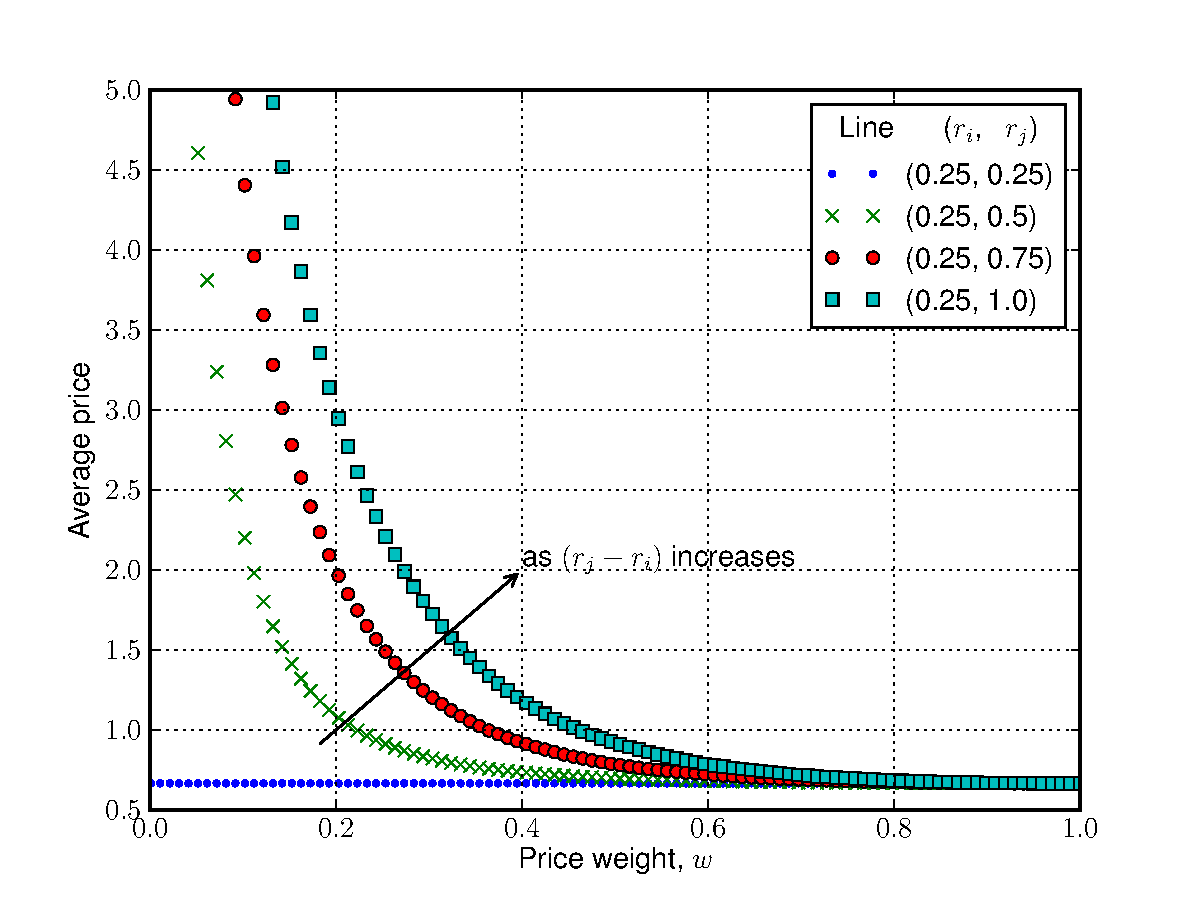
\includegraphics[width=\figsize]{Indirect/Figures/expected_prices}
  \caption{Average prices plotted against the price weight for different pairs of reputation ratings}
  \label{fig:expected_prices_indirect}
  \vspace{10mm}
  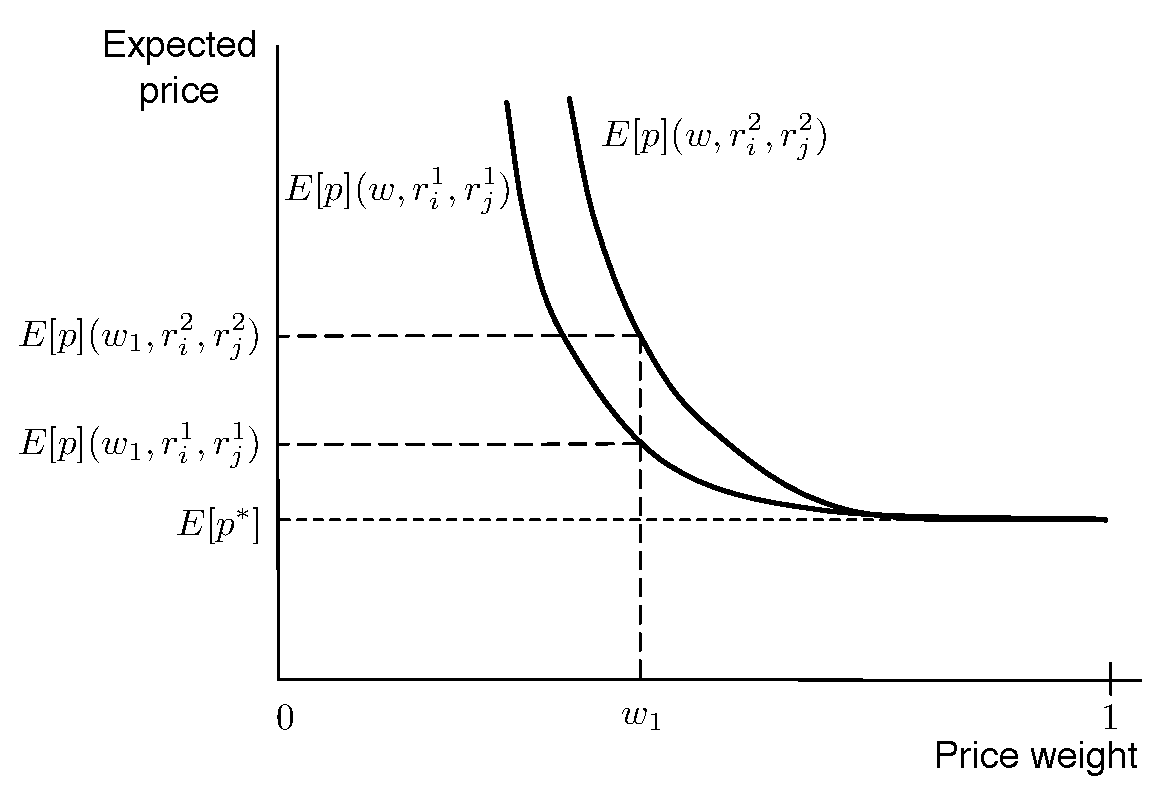
\includegraphics[width=\figsize]{Indirect/Figures/expected_prices_sensitivity}
  \caption{Sensitivity of the price weight to the expected prices}
  \label{fig:expected_prices_sensitivity_indirect}
\end{figure}

\subsection{Subscriber's Perspective: Expected Prices in Restricted Case} % (fold)
\label{sub:subscriber_s_perspective_expected_prices_in_restricted_case_indirect}
Having derived the equilibrium bidding strategy functions in the restricted case, it is possible to examine the expected prices the subscriber will have to pay for different values of the price weight given the reputation ratings of the network operators. We consider only the equilibrium bidding strategy functions in Proposition~\ref{prop:inverse_equi_bidding_str_indirect} since they assume the network operators submit at least their costs. Hence, suppose all of the assumptions of Section~\ref{sec:restricted_case_n_2_indirect} hold; that is, there are two network operators, and costs are uniformly distributed over the interval $[0,1]$. The expected price is equivalent to the expected value of the winning bid; that is, with some abuse of notation
\begin{equation}
  \label{eq:exp_price_def_indirect}
  E[p](w,r_i,r_j) = E[b_i \:\vert\: \arg\min_{i\in N}\beta(w,b_i,r_i)],
\end{equation}
where $b_i$ is the equilibrium bid, and $\beta(w,b_i,r_i) = \beta(b_i,r_i)$ evaluated for a particular value of $w$ for all $i\in N$.

If both network operators have equal reputation ratings, $r = r_i = r_j$ say, then Corollary~\ref{cor:special_case_r_i_r_j_direct} holds for all $w\in [0,1]$. Therefore, regardless of the choice of the price weight, the subscriber expects to pay the price of
\begin{equation}
  \label{eq:exp_price_at_w_1_indirect}
  E[p^*] \equiv E[p](w,r,r) = E\left[\min_{i\in N}\frac{1+c_i}{2}\right] \quad\text{for all } w\in [0,1],
\end{equation}
which is equivalent to Equation~\eqref{eq:standard_fpa_direct} evaluated at $n=2$. In particular, for costs, $c_i$, uniformly distributed over the interval $[0,1]$, $E[p^*] = \frac{2}{3}$.

If, on the other hand, both network operators are characterized by different reputation ratings, then an analytical derivation of the expected prices for each value of the price weight given a pair of reputation ratings is cumbersome. This is due to the fact that network operators bid according to a pair of inverse equilibrium bidding functions specified in Proposition~\ref{prop:inverse_equi_bidding_str_indirect}, which are not easily invertible. Hence, we resort to numerical methods for estimating average (sample mean) prices for selected values of the price weight given a pair of reputation ratings.

To this end, for any given pair of reputation ratings, the costs are pseudo-randomly drawn from the uniform distribution over the discretized interval $[0,1]$. For each selected price weight, the average price is averaged over 10,000 i.i.d.~observations. The Strong Law of Large Numbers (which is stated in Section~\ref{sub:notation_probability_direct}) implies that as the number of observations tends to infinity, the average (sample mean) of the observations approaches the real mean of the distribution of the random variable in question. Therefore, an average of 10,000 observations of the price for each selected price weight should provide a reasonable approximation of the expected price for that price weight. Without loss of generality, suppose further that $r_i \le r_j$. Figure~\ref{fig:expected_prices_indirect} shows the result of the estimation for four pairs of reputation ratings: $(r_i, r_j) = (0.25, 0.25)$, $(0.25, 0.5)$, $(0.25, 0.75)$, and $(0.25, 1.0)$.

It can be observed that regardless of the values of the reputation ratings, the expected prices, $E[p](w,r_i,r_j)$, are bounded from below by $E[p^*]$ for each price weight; this is depicted in Figure~\ref{fig:expected_prices_indirect}. Hence, it can be concluded that regardless of the values of the reputation ratings, the lowest expected price is achieved for $w=1$, and will not decrease as $w$ decreases; in fact, it can only either increase or remain constant.

Furthermore, as the difference $(r_j-r_i)$ increases, the expected prices, $E[p](w,r_i,r_j)$, increase as the price weight decreases; this is depicted in Figure~\ref{fig:expected_prices_indirect}. Therefore, it can be hypothesized that the smaller the difference $(r_j-r_i)$, the less (expected) price sensitive the price weight; that is, for any $w_1\in[0,1]$, if $(r^2_j-r^2_i) > (r^1_j-r^1_i)$ for all $r^1_i,r^1_j,r^2_i,r^2_j\in [0,1]$, then $E[p](w_1,r^2_i,r^2_j) \ge E[p](w_1,r^1_i,r^1_j)$ (Figure~\ref{fig:expected_prices_sensitivity_indirect}). In other words, for any expected price, as the difference $(r_j-r_i)$ between the reputation ratings of the network operators increases, the price weight has to increase (or remain constant) in order to keep the expected price fixed.
% subsection subscriber_s_perspective_expected_prices_in_restricted_case (end)
% section discussion (end)

\section{Bidding Problem Revisited}
\label{sec:bidding_problem_revisited_numerical}
Recall the transformed utility function of each network operator $i\in N$
\begin{equation*}
  u_i(\hat{b},\hat{c}) = \left\{
  \begin{array}{l l}
    \displaystyle\frac{1}{w}\left(\hat{b}_i-\hat{c}_i\right) & \;\text{if } \hat{b}_i < \displaystyle\min_{j\neq i}\hat{b}_j,\\[2ex]
    0 & \;\text{if } \hat{b}_i > \displaystyle\min_{j\neq i}\hat{b}_j,
  \end{array}\right.
\end{equation*}
where $w\neq 0$, and
\begin{equation*}
  \hat{b}_i = wb_i + (1-w)r_i, \quad\text{and}\quad \hat{c}_i = wc_i + (1-w)r_i.
\end{equation*}
In equilibrium, the bids of each network operator equal $\hat{b_i} = \hat{b}_i(\hat{c}_i)$, where $\hat{b}_i$ is the equilibrium bidding function. Denote by $\hat{c}_i(\hat{b}_i)\equiv \hat{b}_i^{-1}(\hat{b}_i)$ an inverse equilibrium bidding function for each network operator $i\in N$. Therefore, the expected utility for each network operator $i\in N$ can be written as
\begin{align*}
  \Pi_i(\hat{b}_i,\hat{c}_i,\hat{b}_{-i},\hat{c}_{-i})
  &\equiv (\hat{b}_i - \hat{c}_i)P\{\text{winning}\mid\hat{b}_i\}\\
  &= (\hat{b}_i - \hat{c}_i)Q_i(\hat{b}_i),
\end{align*}
where
\begin{equation*}
Q_i(\hat{b}_i) = \prod_{j\neq i}\left( 1 - F_j(\hat{c}_j(\hat{b}_i)) \right)
\end{equation*}
is the probability that network operator $i$ is the lowest bidder, and $F_j$ is the distribution function of $\hat{c}_j$.

The first order condition for maximizing network operator $i$'s expected utility is
\begin{equation}
  \label{eq:foc_numerical}
  \frac{d}{d\hat{b}_i}\Pi_i(\hat{b}_i,\hat{c}_i,\hat{b}_{-i},\hat{c}_{-i}) = Q_i(\hat{b}_i) + (\hat{b}_i - \hat{c}_i)\cdot\frac{d}{d\hat{b}_i}Q_i(\hat{b}_i) = 0,
\end{equation}
where
\begin{equation*}
  \frac{d}{d\hat{b}_i}Q_i(\hat{b}_i) = (-1)\sum_{j\neq i} f_j(\hat{c}_j(\hat{b}_i))\frac{d}{d\hat{b}_i}\hat{c}_j(\hat{b}_i)\prod_{k\neq j} \left( 1 - F_k(\hat{c}_k(\hat{b}_i)) \right),
\end{equation*}
and $f_j\equiv\frac{d}{dx}F_j$ (where $x$ is a dummy variable) is the density function of $\hat{c}_j$.

Noting that in equilibrium $\hat{c}_i = \hat{c}_i(\hat{b}_i)$, letting $\hat{b}_i = b$, and rearranging terms in Equation~\eqref{eq:foc_numerical} yields
\begin{align}
  \label{eq:foc_simplified_numerical}
  \frac{1}{b - \hat{c}_i(b)} 
  &= \frac{\sum_{j\neq i} f_j(\hat{c}_j(b))\frac{d}{db}\hat{c}_j(b)\prod_{k\neq j} \left( 1 - F_k(\hat{c}_k(b)) \right)}{\prod_{j\neq i} \left( 1 - F_j(\hat{c}_j(b)) \right)}\nonumber \\[2ex]
  &= \sum_{j\neq i}\frac{f_j(\hat{c}_j(b))}{1 - F_j(\hat{c}_j(b))}\cdot\frac{d}{db}\hat{c}_j(b).
\end{align}
Summing Equation~\eqref{eq:foc_simplified_numerical} over all $n$ network operators yields
\begin{equation}
  \label{eq:foc_summed_numerical}
  \frac{1}{n-1}\sum_{i=1}^n \frac{1}{b - \hat{c}_i(b)} = \sum_{i=1}^n \frac{f_i(\hat{c}_i(b))}{1 - F_i(\hat{c}_i(b))}\cdot\frac{d}{db}\hat{c}_i(b).
\end{equation}
Subtracting Equation~\eqref{eq:foc_simplified_numerical} from \eqref{eq:foc_summed_numerical} yields 
\begin{equation*}
  \frac{1}{n-1}\sum_{i=1}^n \frac{1}{b - \hat{c}_i(b)} - \frac{1}{b - \hat{c}_i(b)} = \frac{f_i(\hat{c}_i(b))}{1 - F_i(\hat{c}_i(b))}\cdot\frac{d}{db}\hat{c}_i(b)
\end{equation*}
which leads to the system of nonlinear ordinary differential equations (ODE)
\begin{equation}
  \label{eq:foc_ode_numerical}
  \frac{d}{db}\hat{c}_i(b) = \frac{1 - F_i(\hat{c}_i(b))}{f_i(\hat{c}_i(b))}\left[ \frac{1}{n-1}\sum_{i=1}^n \frac{1}{b-\hat{c}_i(b)} - \frac{1}{b-\hat{c}_i(b)} \right]
\end{equation}
for $i=1,2,\dotsc,n$.

As pointed out in Section~\ref{sub:indirect_generic_case_static}, Chapter~\ref{cha:network_selection_mechanism_in_the_digital_marketplace}, the derivation of a closed-form solution to the system of ODEs in Equation~\eqref{eq:foc_ode_numerical} is untractable.

\section{Summary}
\label{sec:summary_indirect}

\section{Proofs}
\label{sec:proofs_indirect}
\begin{proof}[Proof of Proposition~\ref{prop:regularity_conditions_indirect}]
Proof of 1) is trivial. To prove 2) and 3), we note that for all $x\in [(1-w)r_i, (1-w)r_i + w]$,
\begin{align*}
  F_i(x)
  &= P\{\hat{C}_i\le x\} \\
  &= P\{wC + (1-w)r_i\le x\} \\
  &= P\left\{ C\le \frac{x - (1-w)r_i}{w} \right\}
\end{align*}
since $\hat{c}_i = wc_i + (1-w)r_i$ and $w\neq 0$. Hence,
\begin{equation*}
  F_i(x) = F_C\left( \frac{x - (1-w)r_i}{w} \right)
\end{equation*}
and
\begin{equation*}
  \frac{x - (1-w)r_i}{w}\in [0,1]
\end{equation*}
for all $x\in [(1-w)r_i, (1-w)r_i + w]$. Therefore, since $F_C$ is differentiable over $(0,1]$ with a derivative $f_C$ locally bounded away from zero over this interval, by extension, $F_i$ is differentiable over $((1-w)r_i, (1-w)r_i + w]$ with a derivative $f_i$ locally bounded away from zero over this interval, and this proves 2). Moreover, since $F_C$ is atomless, by extension, $F_i$ is atomless, and this proves 3).
\end{proof}

\begin{proof}[Proof of Proposition~\ref{prop:characterisation_of_the_equilibrium_indirect}]
Since both $w$ and $r_i$ are assumed to be given to the network operators (i.e., they cannot directly modify their values), the costs-hat and bids-hat are simply convex (and hence, linear) combinations involving costs and bids respectively (Equations~\eqref{eq:b_hat_indirect}~and~\eqref{eq:cost_hat_indirect}). Therefore, a network operator bidding their cost-hat is equivalent to bidding their cost. Hence, to prove 1) we note that Lebrun~\cite{Lebrun2006} proves the existence of a pure-strategy Bayesian Nash equilibrium where network operators submit at least their costs-hat (cf. C.5 Characterization with Possibly Different Lower and Upper Extremities in~\cite{Lebrun2006}). But since costs-hat are equivalent to costs, this also proves the existence of a pure-strategy Bayesian Nash equilibrium where network operators submit at least their costs.

To prove 2) we note that since $r_i\neq r_j$ for at least one network operator $i\in N$ such that $i\neq j$ and $j\in N$, then either $r_i < r_j$ or $r_i > r_j$. Without loss of generality, assume $r_i < r_j$ which implies that $(1-w)r_i < (1-w)r_j$ for all $w\in (0,1)$. By Theorem~1 in Lebrun~\cite{Lebrun2006}, the additional condition (ii) holds, and hence, the considered first-price auction has one and only one pure-strategy Bayesian Nash equilibrium where network operators bid at least their costs-hat. But since costs-hat are equivalent to costs, this also proves the uniqueness of a pure-strategy Bayesian Nash equilibrium where network operators submit at least their costs.
\end{proof}

\begin{proof}[Proof of Proposition~\ref{prop:inverse_equi_bidding_str_indirect}]
The proof is analogous to the proof of Proposition~1 in Kaplan and Zamir~\cite{KaplanZamir2007}.
\end{proof}
